% ----------------------
\chapter{Nota teórica}
% ----------------------
\label{C:nota_teorica}

Un robot omnidireccional es una plataforma que se puede mover autónomamente. Son utilizadas en industrias de manufactura flexibles y en ambientes de servicio \cite{Batlle2009}. Hay tres aspectos importantes que posee un robot omnidireccinal. La figura \ref{F:omni} ayuda a ilustrar las tres características básicas de un rotot omnidireccional.

A continuación, se procede en las siguientes secciones a clarificar algunos conecptos necesarios para entender cómo se consiguen estas características en un robot móvil.

\begin{figure}[H]
    \centering
    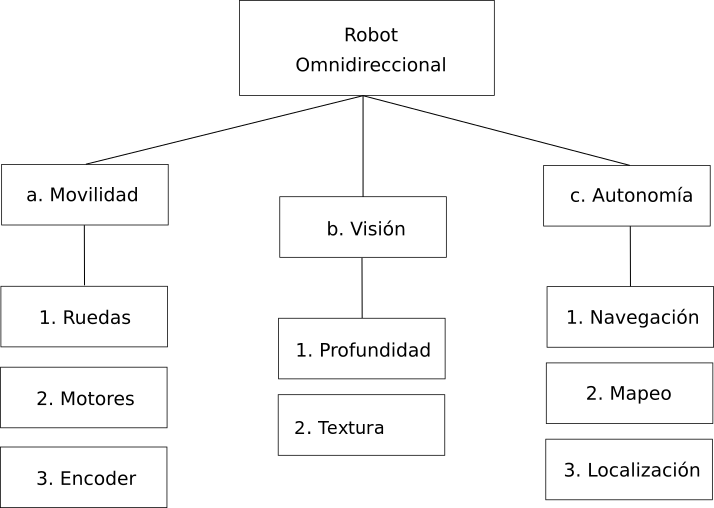
\includegraphics[scale=0.6]{imagenes/robot_omnidireccional.png}
    \caption{Diagrama de componentes de un robot omnidireccional. Autoría propia.}
    \label{F:omni}
\end{figure}


\section{Movilidad}
\subsection{Ruedas}
Existen varios aspectos a considerar cuando se diseña un robot: movilidad, control y posicionamiento. La primera hace referencia a la cantidad de movimientos que un robot puede realizar para llegar a una configuración final. Deben ser capaces de alcanzar cualquier posición y cualquier orientación en su plano de movimiento. Esto quiere decir que el marco del robot debe poseer tres coordenadas independientes del plano general de movimiento \cite{Batlle2009}.

El movimiento se puede realizar con un robot que tiene dos grados de libertad (se puede mover hacia adelante y atrás, con un ángulo de dirección), pero hay que maniobrar. Es más fácil realizar esta tarea si un robot tiene tres grados de libertad. Esto quiere decir, se puede mover hacia adelante y hacia atrás, izquierda derecha, y rotar. De esta manera, la movilidad aumenta, puesto que la cantidad de movimientos posibles que un robot puede realizar para llegar a una configuración final aumenta \cite{Batlle2009}.

Existe un tipo de ruedas, conocidas como ruedas omnidireccionales, que están compuestas de pequeños rodillos que habilitan el deslizamiento de la rueda en cierta dirección. En particular, las ruedas mecanum, como las que se muestran en la figura \ref{F:ruedas_mecanum}, son un caso especial de las ruedas omnidireccionales. Los rodillos están en cierto ángulo $\alpha$ de desface, que permite realizar los movimientos izquierda-derecha con una combinación de fuerzas específica para cada ruedas.

\begin{figure}[H]
  \centering
  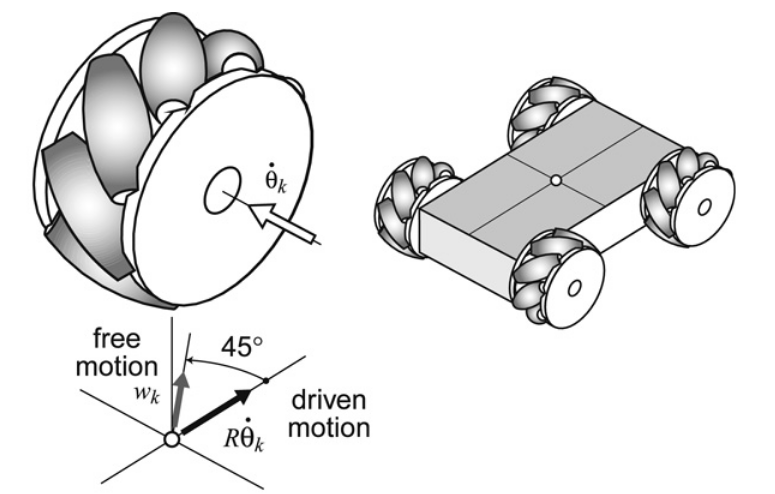
\includegraphics[scale=0.3]{imagenes/ruedas_mecanum.png}
  \caption{Ruedas omnidireccionales Mecanum, con $\alpha = 45^\circ $. Tomado de \cite{Batlle2009}.}
  \label{F:ruedas_mecanum}
\end{figure}

La combinación de las diferentes velocidades en cada uno de los motores, producen los tres grados de libertad en el marco del robot. Específicamene, la kinemática del robot la define el autor \cite{Taheri2015}. A continuación, se muestran las ecuaciones que definen el movimiento del robot:

\begin{equation}
\begin{bmatrix}
w_1\\
w_2\\
w_3\\
w_4\\
\end{bmatrix}
= \frac{1}{r}
\begin{bmatrix}
1 & -1 & -(l_x + l_y) \\
1 & 1 & (l_x + l_y) \\
1 & 1 & -(l_x + l_y) \\
1 & -1 & (l_x + l_y) \\
\end{bmatrix}
\begin{bmatrix}
v_x \\
v_y \\
w_z \\
\end{bmatrix}
\label{E:kinematica_inversa}
\end{equation}

\begin{equation}
\begin{bmatrix}
v_x \\
v_y \\
w_z \\
\end{bmatrix}
= \frac{r}{4}
\begin{bmatrix}
1 & 1 & 1 & 1 \\
-1 & 1 & 1 & -1 \\
\frac{-1}{l_x + l_y} & \frac{1}{l_x + l_y} & \frac{-1}{l_x + l_y} & \frac{1}{l_x + l_y} \\
\end{bmatrix}
\begin{bmatrix}
w_1\\
w_2\\
w_3\\
w_4\\
\label{E:kinematica_directa}
\end{bmatrix}
\end{equation}

\begin{equation}
\begin{bmatrix}
\frac{d v_{x abs}}{dt} \\
\frac{d v_{y abs}}{dt} \\
\end{bmatrix}
 =
\begin{bmatrix}
cos(\frac{d w_z}{d t}) & -sin(\frac{d w_z}{d t}) \\
sin(\frac{d w_z}{d t}) & cos(\frac{d w_z}{d t}) \\
\end{bmatrix}
\begin{bmatrix}
\frac{d v_x}{dt} \\
\frac{d v_y}{dt} \\
\end{bmatrix}
\label{E:transformación}
\end{equation}

La ecuación \ref{E:kinematica_inversa} se utiliza para averiguar la velocidad necesaria en cada una de las ruedas, dado un comando de velocidad relativa al robot. Esto quiere decir que $v_x$ siempre es la velocidad del robot hacia adelante y hacia atrás, sin importar su posición con el mundo. $v_y$ siempre es la velocidad del robot hacia los lados, y lo mismo con $w_Z$.

La ecuación \ref{E:kinematica_directa} en conjunto con la ecuación \ref{E:transformación}, se utilizan para saber la posición real del robot en un plano x,y cartesiano. Es decir, se puede conocer la posición del robot en $x$, $y$, con respecto al mundo.

\subsection{Motores}
Para el robot omnidireccional en contrucción, se utilizarán motores DC. El diagrama básico de un motor DC se muestra en la figura \ref{F:motor_dc}.

\begin{figure}[H]
\centering
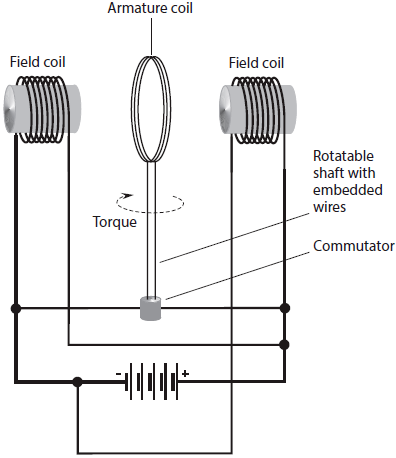
\includegraphics[scale=0.5]{imagenes/motor_dc.png}
\caption{Diagram simplificado de un motor DC. Tomado de \cite{Giblisco2016}}
\label{F:motor_dc}
\end{figure}

Cómo se observa en la figura, en un nivel básico, un motor DC posee dos o más embobinados, los cuáles ejercen una fuerza a un rotor el cuál posee un imán. Cuando pasa una corriente por el embobinado, la bobina produce un campo magnético, que produce una rotación en el rotor. Un comnutador causa que se entrege corriente en diferentes momentos hacia los diferentes embobinados, causando que el rotor gire constantemente \cite{Giblisco2016}.

Cabe destacar que esta conmutación se debe a una característica mecánica de la construcción del motor. Por lo tanto, lo único que se requiere para mover más rápido o más lento el motor, es más corriente o menos. Esto causará que el campo magnético producido sea mayor, y gire el rotor más velozmente.

\subsection{Encoder}
Un encoder es un dispositivo que se encuentra comunmente en sistemas de control modernos, y son utilizados para convertir desplazamiento lineal o rotacional en señales codificadas o pulsos de señal. Los encoders que publican información digital son conocidos como encoders absolutos \cite{Golnaraghi2017}.

Por otra parte, los encoders incrementales, producen un pulso en cada incremento, sin enmbargo no hacen distinción entre los incrementos \cite{Golnaraghi2017}.

En específico, un encoder de quadratura, posee dos sensores a un cierto desfase entre ellos, generalmente de $90^\circ$ . La figura \ref{F:encoder} muestra un ejemplo de un tipo de encoder utilizando luz, y un ejemplo de una señal producida por un encoder incremental de quadratura.

\begin{figure}[H]
\centering
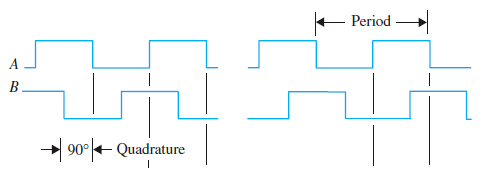
\includegraphics[scale=0.5]{imagenes/encoder_quadratura.png}
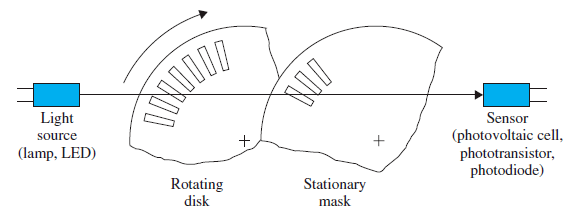
\includegraphics[scale=0.5]{imagenes/encoder_opto.png}
\caption{Ejemplo de un encoder utilizando luz, y la señal producida por un encoder de cuadratura. Tomado de \cite{Golnaraghi2017}.}
\label{F:encoder}
\end{figure}

La señal que se produce, ayuda a identificar la dirección de rotación del motor, ya que el desfase entre las señales proporciona esta información. La frecuencia de los clicks, indican la velocidad del encoder, y finalmente, la cantidad de clicks ayudan a identificar la posición.

\section{Visión}
Para que un robot omnidireccional realice navegación, existe cierta información que resulta ser útil. Los sensores utilizados, generalmente permiten medir dos propiedades del ambiente: la profundidad de lo que se ve (La más importante), y el color de lo que se está viendo. La primera es esencial para lograr la navegación.

\subsection{Profundidad}
Existen muchos tipos de sensores diseñados para dar información de profundidad, como lo son sensores de ultrasonido, sensores laser de rango, entre otros. Sin embargo, la mayoría posee ciertas limitaciones que impiden el uso de los mismos en el campo de los robots autónomos, como lo son los problemas exactitud \cite{DanielMaierArminHornung2012}.

La llegada de los sensores de profundidad en 3D, como el Kinect o el Asus Xtion, que operan com patrones infrarojos han superado estas limitaciones. Estas cámaras son relativamente exactas, y proveen una información densa y tridimensional directamente del hardware \cite{DanielMaierArminHornung2012}. Por esta razón, los mismos sensores son muy utilizados en la navegación de robots autónomos.

Además de sensores como el Kinect, existen sensores de mayor precisión en un ámbito 2D, como lo son los sensores denominados en inglés \textit{Lidar}. Un ejemplo de estos sensores son producidos por la marca Hokuyo.

A continuación se muestra en la figura \ref{F:pointcloud} una muestra de la salida de un sensor de profundidad, utilizando una librería llamada PCL para visualizar la información.

\begin{figure}[H]
\centering
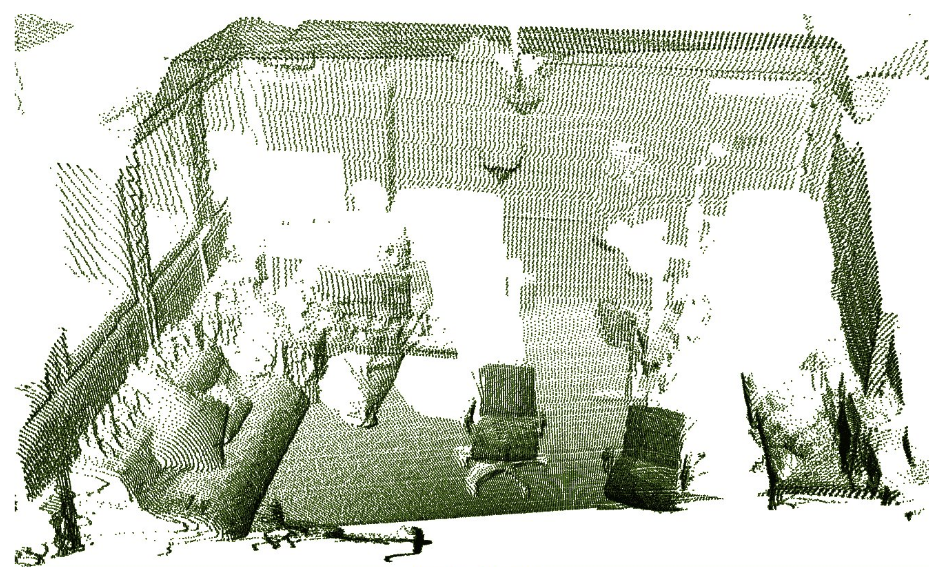
\includegraphics[scale=0.3]{imagenes/rviz_pointcloud.png}
\caption{Imagen de una captura de un sensor de profundidad. Tomado de \cite{Rusu2011}.}
\label{F:pointcloud}
\end{figure}

\subsection{Color}

El color en la parte de visión no es fundamental para realizar navegación. Esta información se puede utilizar para realizar detección de objetos, o encontrar cierto tipo de marcadores en el mundo para ubicarse mejor, sin embargo no es indispensable en el uso de navegación. Ejemplos de casos en donde se utilizan los sensores de color se pueden observar en \cite{Manduchi2005} y \cite{Lai2011}.


\section{Autonomía}

La autonomía en un robot, hace referencia a la capacidad del robot de comportarse de manera ``inteligente'' en algún aspecto \cite{Thrun2005}. Por ejemplo un vehículo que tenga la capacidad de manejarse sólo, y no provoque choques. Otro ejemplo sería robots que puedan limpiar un desastre nuclear, y no sean los humanos los que se vean expuestos a la radiación \cite{Thrun2005}.

Un robot que realice navegación autónomamente, se espera que pueda maniobrar en un espacio, ya sea nuevo o conocido, y pueda crear un mapa del lugar. La navegación por lo tanto, se compone de dos aspectos importantes. El primero, sería el mapeo y el segundo, la localización.

\subsection{Navegación}

Para empezar a diseñar el aspecto de la navegación en un robot, se deben tener principalmente dos cosas. La primera que el robot se pueda mover inteligentemente, y maniobrar lo menos posible. Por lo tanto, un robot que posea tres grados de libertad es deseable, pues hace que la tarea de desplazarse en un ambiente sea bastante sencilla \cite{Batlle2009}.

Además se necesita saber la distancia que ha recorrido el robot en su plano, y cuánto ha rotado. Esto para que el robot sepa que el cambio en la información del sensor de profundidad se debe a un cambio en su posición, y no a un cambio en el mundo. Esto se logra a través de los encoders que se encuentran en los motores del robot.

Finalmente, se necesita un sensor de profundidad, como se habló anteriormente. Esto le permitirá al robot descubrir su entorno, y crear un mapa del mismo.

Existen librerías que contienen la programación necesaria para realizar navegación en un robot que cumpla con los requisitos anteriormente descritos. Un ejemplo, es la librería denominada Navigation Stack, en el entorno de Ros. ROS (Robot Operating System), es un set de librerías, herramientas y convenciones que tratan de simplificar la tarea de crear comportamientos roboticos complejos y robustos a través de una amplia variedad de plataformas robóticas \cite{Quigley2009}.
